\documentclass[10pt,a4paper]{article}
\usepackage[margin=17mm,top=20mm,bottom=19mm]{geometry}
\usepackage[T1]{fontenc}
\usepackage[utf8]{inputenc}
\usepackage{lmodern}
\usepackage{microtype}
\usepackage{amsmath,amssymb,mathtools}
\usepackage{booktabs,tabularx,array,multirow,colortbl}
\usepackage{tikz,pgfplots,pgfplotstable}
\usepgfplotslibrary{groupplots,statistics,fillbetween}
\usetikzlibrary{arrows.meta,positioning,calc,shapes.geometric,decorations.pathreplacing}
\usepackage{tcolorbox}
\tcbuselibrary{skins,breakable}
\usepackage{fancyhdr,lastpage,enumitem,hyperref,xcolor}
\pgfplotsset{compat=1.18}
\definecolor{paper}{HTML}{FAFAF8}
\definecolor{ink}{HTML}{202D30}
\definecolor{muted}{HTML}{657371}
\definecolor{line}{HTML}{D6DEDA}
\definecolor{sage}{HTML}{578B7B}
\definecolor{sagewash}{HTML}{DFECE5}
\definecolor{mint}{HTML}{B9D4C8}
\definecolor{teal}{HTML}{206D70}
\definecolor{coral}{HTML}{D87954}
\definecolor{slate}{HTML}{566477}
\definecolor{silver}{HTML}{9BABA7}
\definecolor{gold}{HTML}{C49B51}
\definecolor{bad}{HTML}{B65954}
\pagecolor{paper}
\color{ink}
\hypersetup{colorlinks=true,urlcolor=teal,linkcolor=teal,pdftitle={RELAY Final QA and Benchmark Report},pdfauthor={RELAY Research and Engineering QA}}
\setlength{\parskip}{5pt}
\setlength{\parindent}{0pt}
\renewcommand{\arraystretch}{1.15}
\setlist[itemize]{leftmargin=1.5em,itemsep=2pt,topsep=3pt}
\pagestyle{fancy}
\fancyhf{}
\fancyhead[L]{\footnotesize\sffamily\bfseries RELAY / FINAL QUALITY ASSESSMENT}
\fancyhead[R]{\footnotesize\sffamily\color{muted} Research benchmark / Synthetic}
\fancyfoot[L]{\footnotesize\color{muted} Source: v10/v11 QA and independent hybrid holdout}
\fancyfoot[R]{\footnotesize\color{muted}\thepage\ / \pageref{LastPage}}
\renewcommand{\headrulewidth}{0.3pt}
\renewcommand{\footrulewidth}{0pt}
\setlength{\headheight}{13pt}
\newcommand{\sect}[2]{\vspace{4mm}{\Large\sffamily\bfseries #1}\hfill{\small\sffamily\color{muted}#2}\par\vspace{1mm}\color{sage}\rule{\linewidth}{1.0pt}\color{ink}\vspace{2mm}}
\newcommand{\subsect}[1]{\vspace{3mm}{\large\sffamily\bfseries #1}\par\vspace{1mm}}
\newcommand{\methodnote}[1]{{\footnotesize\color{muted}\textit{#1}}\par}
\newcommand{\good}[1]{{\bfseries\color{teal}#1}}
\newcommand{\risk}[1]{{\bfseries\color{bad}#1}}
\newtcolorbox{insight}[1][]{enhanced,breakable,colback=sagewash,colframe=sagewash,arc=2mm,boxrule=0pt,left=3mm,right=3mm,top=2mm,bottom=2mm,#1}
\newtcolorbox{caution}[1][]{enhanced,breakable,colback=coral!8,colframe=coral!25,arc=2mm,boxrule=.4pt,left=3mm,right=3mm,top=2mm,bottom=2mm,#1}
\pgfplotsset{replot/.style={width=\linewidth,height=6.3cm,axis background/.style={fill=white},grid=major,grid style={line!70},axis line style={muted!80},tick style={draw=none},tick label style={font=\scriptsize,color=muted},label style={font=\small,color=ink},title style={font=\small\bfseries,color=ink},legend style={draw=none,fill=white,font=\scriptsize,at={(0.5,-0.23)},anchor=north,legend columns=-1},bar width=7pt,scaled ticks=false}}
\pgfplotsset{cleanbar/.style={replot,ybar,bar width=8pt,enlarge x limits=0.14,axis x line*=bottom,axis y line*=left}}
\newcommand{\smallcaps}[1]{{\sffamily\small\bfseries\color{sage}#1}}
\begin{document}

% ---------------------------- COVER -------------------------------
\vspace*{9mm}
{\sffamily\small\bfseries\color{sage} ENGINEERING RESEARCH / FINAL RELEASE EVIDENCE }\hfill {\sffamily\small\color{muted} 11 November 2026}\par\vspace{6mm}
{\sffamily\fontsize{30}{34}\selectfont\bfseries RELAY}\par\vspace{1mm}
{\sffamily\fontsize{20}{25}\selectfont Final QA, Benchmark\\and Economic Value Assessment}\par\vspace{4mm}
{\large\color{muted} Five dispatch policies, six operating regimes, risk--quality--cost frontiers, statistical convergence, and deployment readiness.}\par\vspace{9mm}

\begin{tikzpicture}
\fill[sagewash] (0,0) rectangle (\linewidth,0.2); % decorative rule is resized by TeX dimension
\end{tikzpicture}\par
\begin{minipage}[t]{0.245\linewidth}
\begin{tcolorbox}[colback=white,colframe=line,arc=2mm,boxrule=.4pt,height=29mm]
{\footnotesize\color{muted} Strategies tested}\par\vspace{2mm}{\LARGE\bfseries 5}\par\vspace{1mm}{\scriptsize FCFS to RELAY hybrids}
\end{tcolorbox}
\end{minipage}\hfill
\begin{minipage}[t]{0.245\linewidth}
\begin{tcolorbox}[colback=white,colframe=line,arc=2mm,boxrule=.4pt,height=29mm]
{\footnotesize\color{muted} Operating regimes}\par\vspace{2mm}{\LARGE\bfseries 6}\par\vspace{1mm}{\scriptsize Paired synthetic trials}
\end{tcolorbox}
\end{minipage}\hfill
\begin{minipage}[t]{0.245\linewidth}
\begin{tcolorbox}[colback=white,colframe=line,arc=2mm,boxrule=.4pt,height=29mm]
{\footnotesize\color{muted} Shared episodes}\par\vspace{2mm}{\LARGE\bfseries 3,000}\par\vspace{1mm}{\scriptsize Holdout seed 9099}
\end{tcolorbox}
\end{minipage}\hfill
\begin{minipage}[t]{0.245\linewidth}
\begin{tcolorbox}[colback=white,colframe=line,arc=2mm,boxrule=.4pt,height=29mm]
{\footnotesize\color{muted} Policy outcomes}\par\vspace{2mm}{\LARGE\bfseries 15,000}\par\vspace{1mm}{\scriptsize 500 per regime and policy}
\end{tcolorbox}
\end{minipage}
\vspace{5mm}
\begin{insight}
{\sffamily\bfseries KEY RESULT --- NORMAL CONDITIONS (HYBRID HOLDOUT)}\par
\vspace{3mm}
\begin{tabularx}{\linewidth}{@{}XXX@{}}
\good{11.47\%} cost reduction & \good{64.05\%} on-time rate & \good{14.40\%} lower CVaR$_{90}$\\
RELAY + Model A vs FCFS & FCFS: 39.36\% & Worst-decile episode cost
\end{tabularx}
\vspace{2mm}
\methodnote{All three figures are from synthetic ground-staging episodes, not from live airline operations. Real-world monetary ROI has not been measured.}
\end{insight}
\vspace{3mm}
\begin{caution}
\textbf{Scientific scope.} This is a reproducible benchmark of \emph{ground-staging dispatch policies}, with supporting QA of RELAY's three mathematical modules and twin interfaces. It is \emph{not} an empirical validation of Cathay Cargo savings, aircraft-certified ULD loading, full joint optimisation, or a deployed production system.
\end{caution}
\newpage

% ------------------------- EXECUTIVE SUMMARY ----------------------
\sect{01 / Executive evidence summary}{RESULTS AT A GLANCE}
\begin{tabularx}{\linewidth}{@{}p{40mm}Xr@{}}
\toprule
\textbf{Claim} & \textbf{Actual evidence} & \textbf{Status}\\\midrule
Software regression & v10: 124/124 tests in three groups; v11: 56/56 selected tests; groups overlap & Tested\\
Ground policy quality & 15,000 policy outcomes on 3,000 common episodes; six scenarios & Tested\\
Original model mathematics & Bounded 2D ULD; one-step Bayes; finite-column MILP & Partial\\
Three Twin consistency & Shared IDs, event state and simulated clock; API flows exercised & Tested\\
Safety certification & No operator-approved 3D contour, restraint or live booking authority & Not proven\\
Live airline economics & No licensed operational cost ledger or field experiment & Not measured\\
\bottomrule
\end{tabularx}
\vspace{4mm}
\begin{insight}
\textbf{What the evidence supports.} The new policy family reduces synthetic penalty cost and improves service quality in several regimes. Normal-operation RELAY + Model A lowers average cost \textbf{11.47\%} versus FCFS while raising the on-time rate by \textbf{24.69 percentage points}. A cost-first EDF variant saves \textbf{17.53\%}, but has a lower on-time rate (\textbf{56.64\%}). The difference exposes a real multi-objective trade-off within the simulator.
\end{insight}
\subsect{Policies under comparison}
\begin{tabularx}{\linewidth}{@{}p{34mm}X@{}}
\toprule
FCFS & First-come, first-served reference policy.\\
RELAY v10 & Original urgency-weighted staging policy.\\
RELAY v11 & Duration, priority and deadline-aware triage, with conservative low-crew fallback.\\
RELAY + Model A & Experimental \textbf{DeadlineGuard-A} hybrid; more explicit protection for urgent and critical jobs. \textbf{Not an external LLM.}\\
RELAY + EDF & Experimental cost-first earliest-deadline dispatch variant.\\
\bottomrule
\end{tabularx}
\subsect{Independent experiment identities}
\begin{tabularx}{\linewidth}{@{}p{29mm}p{24mm}p{24mm}X@{}}
\toprule
\textbf{Dataset} & \textbf{Seed} & \textbf{Size} & \textbf{Proper interpretation}\\\midrule
Legacy v10 QA & Prior v10 setup & 5 $\times$ 500 & 21-tick window, incomplete work may bias apparent performance.\\
v11 cohort & 2026 & 6 $\times$ 500 & 24-tick arrivals + up to 110 clearance ticks, with remaining jobs accounted for.\\
Hybrid holdout & 9099 & 6 $\times$ 500 & Five policies on common episodes; main head-to-head rankings.\\
\bottomrule
\end{tabularx}
\begin{caution}
\textbf{No cross-cohort subtraction.} v11 results measured with seed 2026 must not be subtracted directly from hybrid holdout results with seed 9099 as if they were matched trials. All policy rankings below use the \textbf{same holdout seed 9099} unless explicitly labelled otherwise.
\end{caution}
\newpage

% ------------------------- NORMAL RANKING -------------------------
\sect{02 / Head-to-head leaderboard}{HOLDOUT / NORMAL CONDITIONS}
\begin{tabularx}{\linewidth}{@{}>{\raggedright\arraybackslash}p{40mm}rrrr@{}}
\toprule
\textbf{Policy} & \textbf{On-time} & \textbf{Cost} & \textbf{Cost saved} & \textbf{CVaR$_{90}$ saved}\\\midrule
FCFS & 39.36\% & 1,946.84 & --- & ---\\
RELAY v10 & 36.41\% & 1,820.14 & 6.51\% & 2.67\%\\
RELAY v11 & 64.02\% & 1,775.19 & 8.82\% & 12.20\%\\
\rowcolor{sagewash} \textbf{RELAY + Model A} & \textbf{64.05\%} & \textbf{1,723.60} & \textbf{11.47\%} & \textbf{14.40\%}\\
RELAY + EDF & 56.64\% & 1,605.65 & \textbf{17.53\%} & \textbf{18.87\%}\\
\bottomrule
\end{tabularx}
\methodnote{Cost is synthetic penalty units per episode; lower is better. On-time rate and CVaR are measured over synthetic episodes; higher savings percentages are better.}
\vspace{4mm}
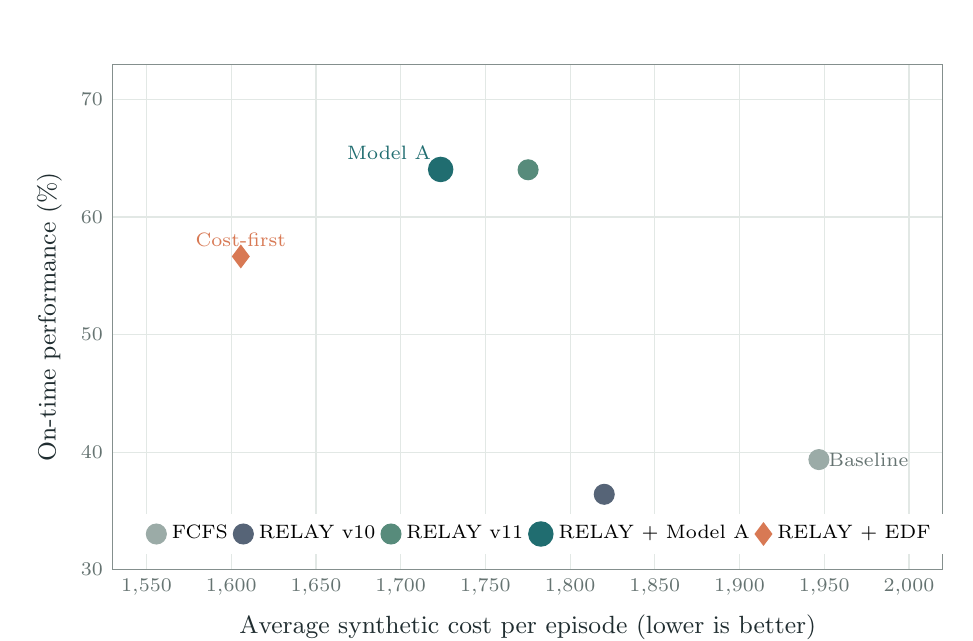
\begin{tikzpicture}
\begin{axis}[replot,width=\linewidth,height=8cm,xmin=1530,xmax=2020,ymin=30,ymax=73,xlabel={Average synthetic cost per episode (lower is better)},ylabel={On-time performance (\%)},legend pos=south west,legend style={font=\scriptsize,draw=none,fill=white}]
\addplot[only marks,mark=*,mark size=3.6pt,color=silver] coordinates {(1946.835,39.359)};\addlegendentry{FCFS}
\addplot[only marks,mark=*,mark size=3.6pt,color=slate] coordinates {(1820.142,36.407)};\addlegendentry{RELAY v10}
\addplot[only marks,mark=*,mark size=3.6pt,color=sage] coordinates {(1775.193,64.018)};\addlegendentry{RELAY v11}
\addplot[only marks,mark=*,mark size=4.4pt,color=teal] coordinates {(1723.600,64.045)};\addlegendentry{RELAY + Model A}
\addplot[only marks,mark=diamond*,mark size=4pt,color=coral] coordinates {(1605.648,56.640)};\addlegendentry{RELAY + EDF}
\node[anchor=south east,font=\scriptsize,color=teal] at (axis cs:1723.6,64.045) {Model A};
\node[anchor=south,font=\scriptsize,color=coral] at (axis cs:1605.648,56.64) {Cost-first};
\node[anchor=west,font=\scriptsize,color=muted] at (axis cs:1946.835,39.359) {Baseline};
\end{axis}
\end{tikzpicture}\par
\methodnote{Benchmark analogue of an LLM accuracy-vs-cost curve: up-and-left is preferable. Policies are points, not continuous cost/accuracy tuning curves.}
\newpage

% ------------------------- SCENARIO COST --------------------------
\sect{03 / Six-regime cost benchmark}{SYNTHETIC HOLDOUT / SEED 9099}
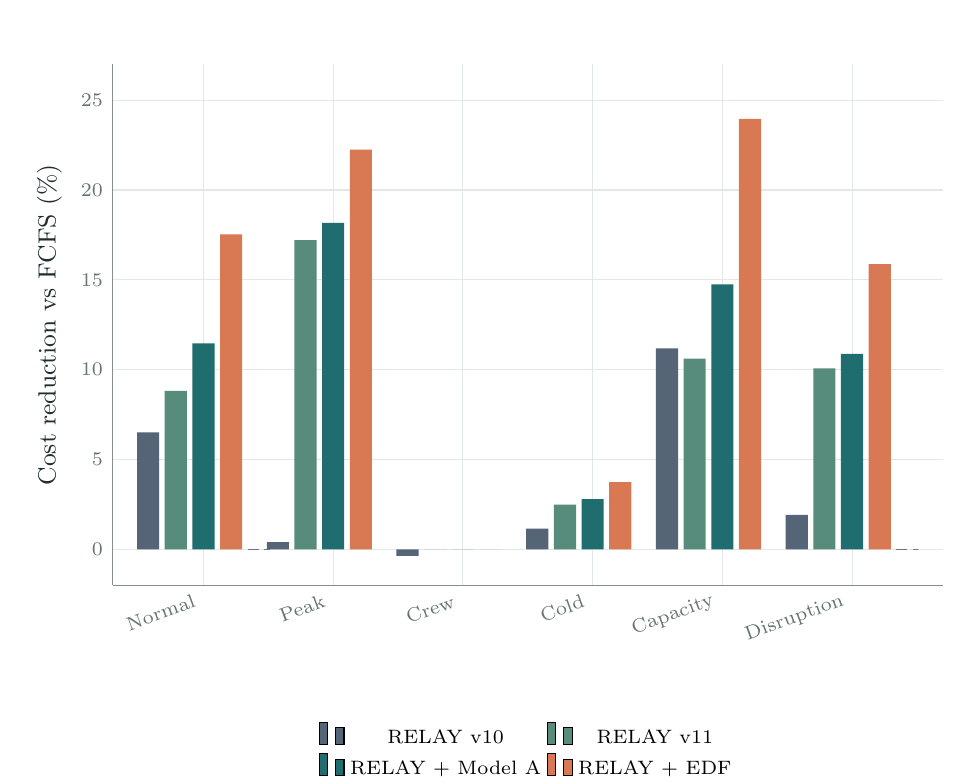
\begin{tikzpicture}
\begin{axis}[cleanbar,width=\linewidth,height=8.2cm,symbolic x coords={Normal,Peak,Crew,Cold,Capacity,Disruption},xtick=data,x tick label style={font=\scriptsize,rotate=20,anchor=east},ylabel={Cost reduction vs FCFS (\%)},ymin=-2,ymax=27,legend style={at={(0.5,-0.25)},anchor=north,legend columns=2,font=\scriptsize}]
\addplot[fill=slate,draw=none] coordinates {(Normal,6.508)(Peak,0.403)(Crew,-0.366)(Cold,1.152)(Capacity,11.192)(Disruption,1.928)};\addlegendentry{RELAY v10}
\addplot[fill=sage,draw=none] coordinates {(Normal,8.816)(Peak,17.216)(Crew,0)(Cold,2.496)(Capacity,10.616)(Disruption,10.073)};\addlegendentry{RELAY v11}
\addplot[fill=teal,draw=none] coordinates {(Normal,11.467)(Peak,18.175)(Crew,0)(Cold,2.794)(Capacity,14.749)(Disruption,10.879)};\addlegendentry{RELAY + Model A}
\addplot[fill=coral,draw=none] coordinates {(Normal,17.525)(Peak,22.240)(Crew,0)(Cold,3.737)(Capacity,23.953)(Disruption,15.881)};\addlegendentry{RELAY + EDF}
\addplot[black!55,dashed,no marks,domain=-1:8] coordinates {(Normal,0)(Disruption,0)};
\end{axis}
\end{tikzpicture}\par\vspace{2mm}
\begin{tabularx}{\linewidth}{@{}lrrrr@{}}
\toprule
\textbf{Regime} & \textbf{v10} & \textbf{v11} & \textbf{Model A} & \textbf{EDF}\\\midrule
Normal & 6.51\% & 8.82\% & 11.47\% & \textbf{17.53\%}\\
Peak demand & 0.40\% & 17.22\% & 18.18\% & \textbf{22.24\%}\\
Crew shortage & \risk{--0.37\%} & 0.00\% & 0.00\% & 0.00\%\\
Cold outage & 1.15\% & 2.50\% & 2.79\% & \textbf{3.74\%}\\
High capacity & 11.19\% & 10.62\% & 14.75\% & \textbf{23.95\%}\\
Temporary disruption & 1.93\% & 10.07\% & 10.88\% & \textbf{15.88\%}\\
\bottomrule
\end{tabularx}
\begin{insight}
\textbf{Why EDF is not an automatic winner.} EDF obtains the lowest synthetic cost in all six holdout regimes, but the quality metric differs. In peak demand it achieves 28.84\% on-time versus 39.31\% for Model A; the 10.47 percentage-point gap is operationally meaningful even though EDF is cheaper under the synthetic penalty schedule.
\end{insight}
\newpage

% ------------------------- QUALITY PROFILE -----------------------
\sect{04 / Service-quality comparison}{WHAT COST ALONE HIDES}
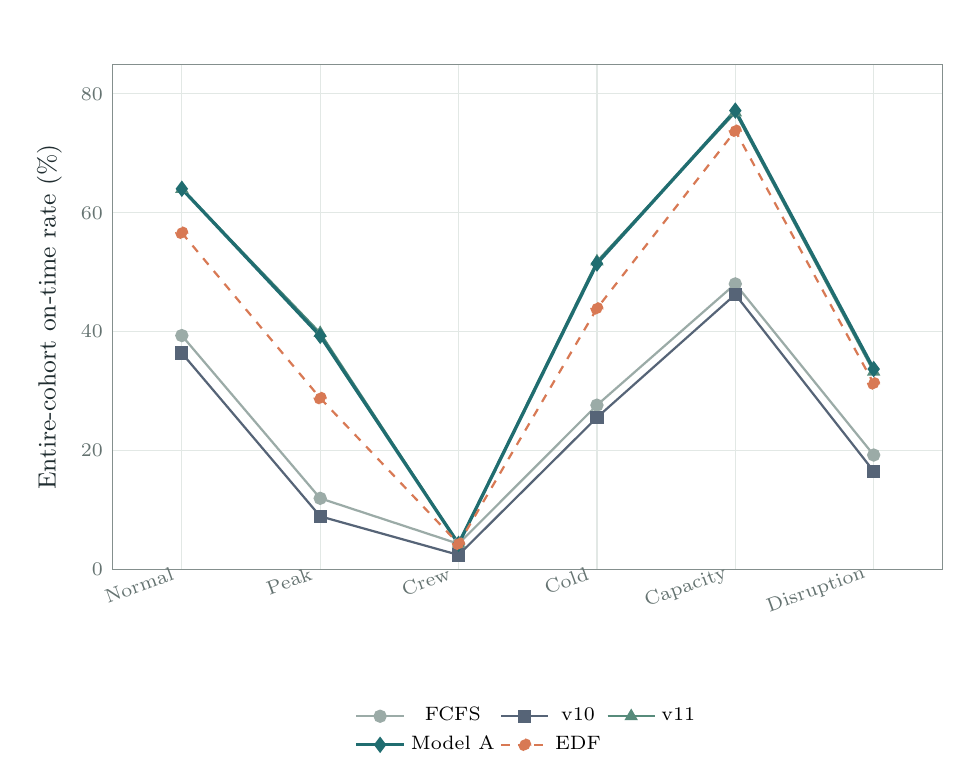
\begin{tikzpicture}
\begin{axis}[replot,width=\linewidth,height=8cm,symbolic x coords={Normal,Peak,Crew,Cold,Capacity,Disruption},xtick=data,x tick label style={rotate=20,anchor=east,font=\scriptsize},ylabel={Entire-cohort on-time rate (\%)},ymin=0,ymax=85,legend style={at={(0.5,-0.25)},anchor=north,legend columns=3}]
\addplot[mark=*,thick,color=silver] coordinates {(Normal,39.359)(Peak,11.986)(Crew,4.331)(Cold,27.655)(Capacity,48.048)(Disruption,19.267)};\addlegendentry{FCFS}
\addplot[mark=square*,thick,color=slate] coordinates {(Normal,36.407)(Peak,8.956)(Crew,2.464)(Cold,25.576)(Capacity,46.273)(Disruption,16.544)};\addlegendentry{v10}
\addplot[mark=triangle*,thick,color=sage] coordinates {(Normal,64.018)(Peak,39.788)(Crew,4.331)(Cold,51.825)(Capacity,76.885)(Disruption,33.286)};\addlegendentry{v11}
\addplot[mark=diamond*,very thick,color=teal] coordinates {(Normal,64.045)(Peak,39.306)(Crew,4.331)(Cold,51.475)(Capacity,77.195)(Disruption,33.728)};\addlegendentry{Model A}
\addplot[mark=*,dashed,thick,color=coral] coordinates {(Normal,56.640)(Peak,28.839)(Crew,4.331)(Cold,43.918)(Capacity,73.801)(Disruption,31.304)};\addlegendentry{EDF}
\end{axis}
\end{tikzpicture}\par
\subsect{Normal-operation quality decomposition}
\begin{tabularx}{\linewidth}{@{}Xrrr@{}}
\toprule
\textbf{Metric} & \textbf{FCFS} & \textbf{Model A} & \textbf{Improvement}\\\midrule
On-time rate & 39.359\% & 64.045\% & +24.686 pp\\
Mean synthetic cost & 1,946.835 & 1,723.600 & 11.467\% lower\\
Average lead time & 11.623 ticks & 11.224 ticks & 3.428\% lower\\
Worst-decile cost (CVaR$_{90}$) & Baseline & Measured & 14.396\% lower\\
Episodes worse than FCFS & --- & 13.0\% & Not zero\\
\bottomrule
\end{tabularx}
\methodnote{A percentage-point change (pp) is not a relative percentage change: $64.045-39.359=24.686$ pp. The corresponding relative increase in the on-time rate is approximately 62.72\%.}
\newpage

% ------------------------- TAIL AND DOWNSIDE ---------------------
\sect{05 / Downside and tail risk}{MEAN BENEFIT IS NOT A GUARANTEE}
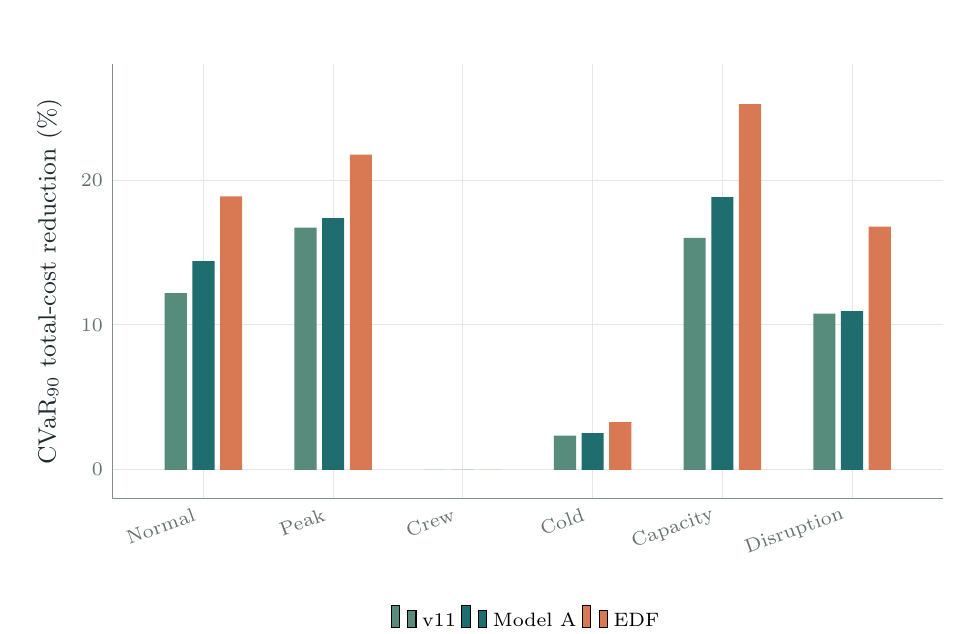
\begin{tikzpicture}
\begin{axis}[cleanbar,width=\linewidth,height=7.1cm,symbolic x coords={Normal,Peak,Crew,Cold,Capacity,Disruption},xtick=data,x tick label style={rotate=20,anchor=east,font=\scriptsize},ylabel={CVaR$_{90}$ total-cost reduction (\%)},ymin=-2,ymax=28,legend style={at={(0.5,-0.23)},anchor=north,legend columns=3}]
\addplot[fill=sage,draw=none] coordinates {(Normal,12.196)(Peak,16.710)(Crew,0)(Cold,2.350)(Capacity,16.010)(Disruption,10.778)};\addlegendentry{v11}
\addplot[fill=teal,draw=none] coordinates {(Normal,14.396)(Peak,17.377)(Crew,0)(Cold,2.526)(Capacity,18.822)(Disruption,10.945)};\addlegendentry{Model A}
\addplot[fill=coral,draw=none] coordinates {(Normal,18.874)(Peak,21.760)(Crew,0)(Cold,3.284)(Capacity,25.238)(Disruption,16.794)};\addlegendentry{EDF}
\end{axis}
\end{tikzpicture}\par\vspace{2mm}
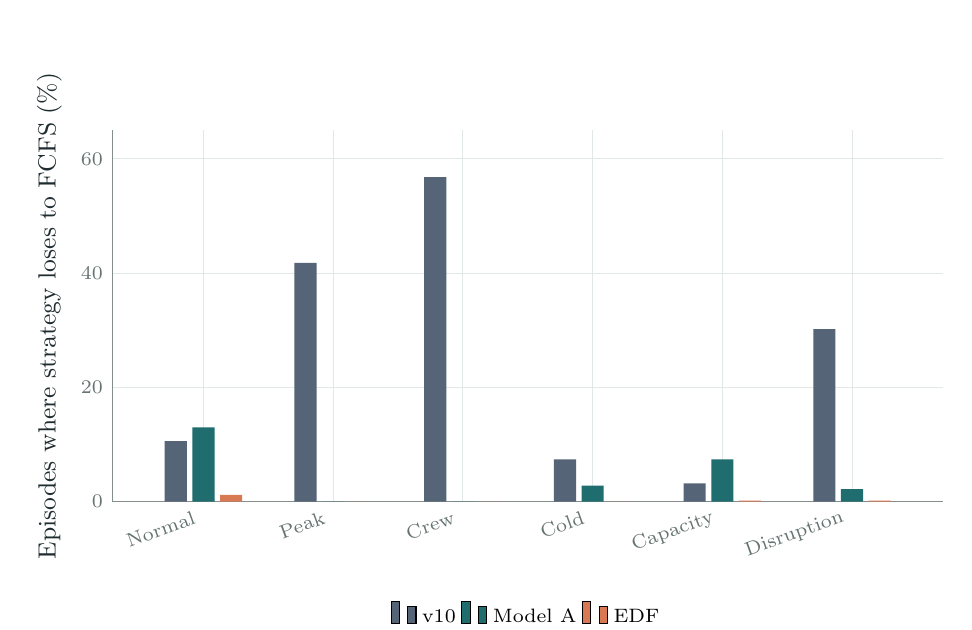
\begin{tikzpicture}
\begin{axis}[cleanbar,width=\linewidth,height=6.3cm,symbolic x coords={Normal,Peak,Crew,Cold,Capacity,Disruption},xtick=data,x tick label style={rotate=20,anchor=east,font=\scriptsize},ylabel={Episodes where strategy loses to FCFS (\%)},ymin=0,ymax=65,legend style={at={(0.5,-0.25)},anchor=north,legend columns=3}]
\addplot[fill=slate,draw=none] coordinates {(Normal,10.6)(Peak,41.8)(Crew,56.8)(Cold,7.4)(Capacity,3.2)(Disruption,30.2)};\addlegendentry{v10}
\addplot[fill=teal,draw=none] coordinates {(Normal,13.0)(Peak,0)(Crew,0)(Cold,2.8)(Capacity,7.4)(Disruption,2.2)};\addlegendentry{Model A}
\addplot[fill=coral,draw=none] coordinates {(Normal,1.2)(Peak,0)(Crew,0)(Cold,0)(Capacity,0.2)(Disruption,0.2)};\addlegendentry{EDF}
\end{axis}
\end{tikzpicture}\par
\begin{caution}
Tail cost risk is calculated across complete synthetic episodes. The Model III CVaR for correlated flight scenarios is a \emph{different random variable} and is not numerically interchangeable with these staging-policy CVaR values. A lower average cost does not certify an airline safety or SLA constraint.
\end{caution}
\newpage

% ------------------------- CONVERGENCE ---------------------------
\sect{06 / Statistical convergence}{500 PAIRED EPISODES}
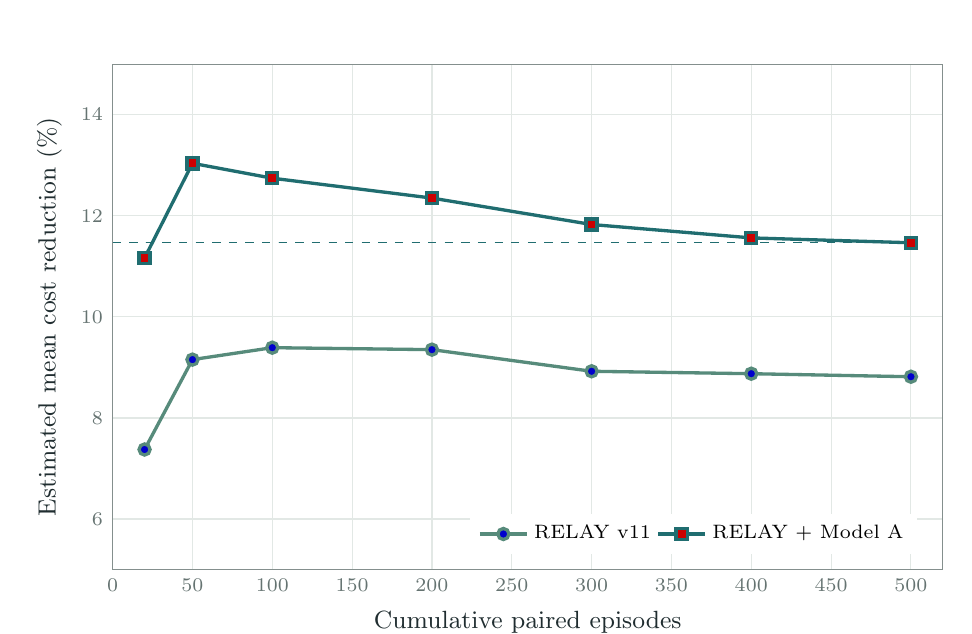
\begin{tikzpicture}
\begin{axis}[replot,width=\linewidth,height=8cm,xmin=0,xmax=520,ymin=5,ymax=15,xlabel={Cumulative paired episodes},ylabel={Estimated mean cost reduction (\%)},legend pos=south east]
\addplot+[very thick,color=sage,mark=*,mark size=2pt] coordinates {(20,7.376)(50,9.155)(100,9.391)(200,9.352)(300,8.924)(400,8.876)(500,8.816)};\addlegendentry{RELAY v11}
\addplot+[very thick,color=teal,mark=square*,mark size=2pt] coordinates {(20,11.166)(50,13.039)(100,12.744)(200,12.351)(300,11.828)(400,11.563)(500,11.467)};\addlegendentry{RELAY + Model A}
\addplot[color=teal,dashed,no marks,domain=0:500] {11.467};
\end{axis}
\end{tikzpicture}\par\vspace{2mm}
\begin{tabularx}{\linewidth}{@{}lrrrrrrr@{}}
\toprule
Episodes & 20 & 50 & 100 & 200 & 300 & 400 & 500\\\midrule
v11 saving (\%) & 7.38 & 9.16 & 9.39 & 9.35 & 8.92 & 8.88 & 8.82\\
Model A saving (\%) & 11.17 & 13.04 & 12.74 & 12.35 & 11.83 & 11.56 & 11.47\\
\bottomrule
\end{tabularx}
\begin{insight}
\textbf{Bootstrap uncertainty, normal holdout.} RELAY v11: 8.82\% cost reduction (95\% paired bootstrap CI \textbf{7.95--9.59\%}); Model A: 11.47\% (\textbf{10.69--12.21\%}). Model A's additional saving relative to v11's synthetic cost is about \textbf{2.91\%} under this common test set.
\end{insight}
\methodnote{The 500-episode curves demonstrate Monte Carlo estimator stabilisation, not convergence of the optimisation solver, proof of generalisation, or real operational performance. Repeated looks at the same sampled episodes are correlated.}
\newpage

% ------------------------- DATA AND FREQUENCY --------------------
\sect{07 / Input-data QA and frequency}{GENERATOR VALIDATION}
\begin{tabularx}{\linewidth}{@{}Xrrrr@{}}
\toprule
Dataset & Flights & Shipments & Pieces & Events\\\midrule
30-day synthetic history & \textbf{429} & \textbf{636} & \textbf{793} & \textbf{5,120}\\
\bottomrule
\end{tabularx}
\methodnote{Also 14 synthetic ULD records. No observed duplicates or broken shipment--piece references in the completed v10 QA checks. This measures structural consistency, not ground truth realism.}
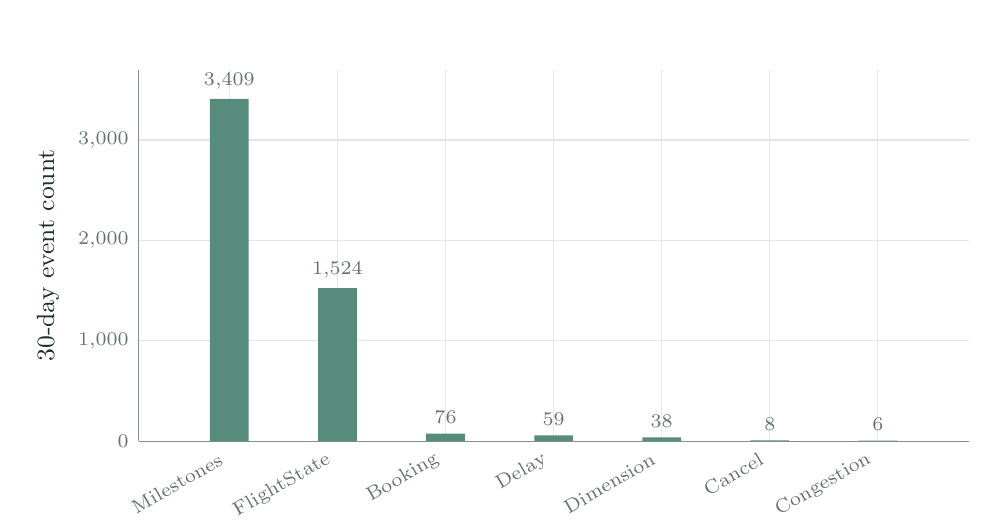
\begin{tikzpicture}
\begin{axis}[cleanbar,width=\linewidth,height=6.3cm,symbolic x coords={Milestones,FlightState,Booking,Delay,Dimension,Cancel,Congestion},xtick=data,x tick label style={rotate=30,anchor=east,font=\scriptsize},ylabel={30-day event count},ymin=0,ymax=3700,bar width=14pt]
\addplot[fill=sage,draw=none,nodes near coords,point meta=y,nodes near coords style={font=\scriptsize,color=muted,rotate=0,anchor=south}] coordinates {(Milestones,3409)(FlightState,1524)(Booking,76)(Delay,59)(Dimension,38)(Cancel,8)(Congestion,6)};
\end{axis}
\end{tikzpicture}\par
\subsect{Synthetic arrival-process validation}
\begin{minipage}{.56\linewidth}
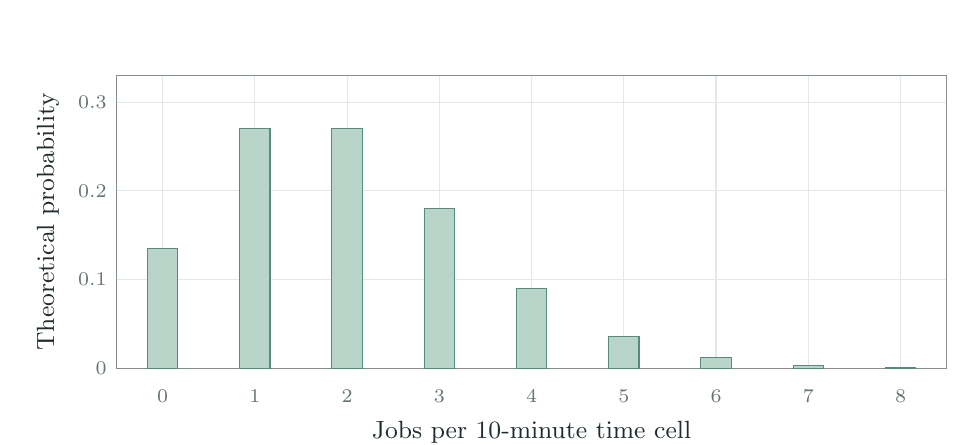
\begin{tikzpicture}
\begin{axis}[replot,width=\linewidth,height=5.3cm,ybar,bar width=11pt,xmin=-0.5,xmax=8.5,ymin=0,ymax=.33,xtick={0,1,2,3,4,5,6,7,8},xlabel={Jobs per 10-minute time cell},ylabel={Theoretical probability}]
\addplot[fill=mint,draw=sage] coordinates {(0,.135335)(1,.270671)(2,.270671)(3,.180447)(4,.090224)(5,.036089)(6,.012030)(7,.003437)(8,.000859)};
\end{axis}
\end{tikzpicture}\par
\end{minipage}\hfill
\begin{minipage}{.40\linewidth}
\begin{tcolorbox}[colback=white,colframe=line,arc=2mm]
{\scriptsize\color{muted} Normal scenario / Poisson generator}\par\vspace{2mm}
$\lambda=2.000$ jobs per cell\\
\textbf{12,000} observed cells\\
Observed mean: \textbf{1.9725}\\
Observed variance: \textbf{1.9589}\\
\vspace{2mm}
$P(N=k)=\mathrm e^{-2}\,2^k/k!$
\end{tcolorbox}
\end{minipage}
\methodnote{Plot shows the \emph{theoretical} Poisson($2$) probability mass function, not an empirical frequency histogram; only measured mean and variance were retained for the present audit. A distribution can be internally well-implemented yet poorly calibrated to a real cargo terminal.}
\newpage

% ------------------------- THREE MODEL QA ------------------------
\sect{08 / Mathematical QA traceability}{THREE RESEARCH LAYERS}
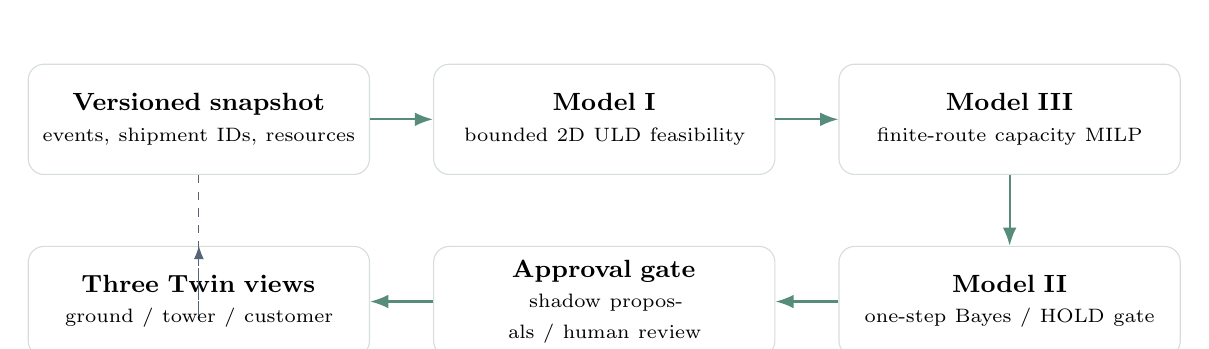
\begin{tikzpicture}[node distance=7mm,>=Latex]
\tikzset{nodebox/.style={draw=line,rounded corners=2mm,fill=white,minimum height=14mm,text width=41mm,align=center,font=\small}}
\node[nodebox] (s) {\textbf{Versioned snapshot}\\\scriptsize events, shipment IDs, resources};
\node[nodebox,right=8mm of s] (i) {\textbf{Model I}\\\scriptsize bounded 2D ULD feasibility};
\node[nodebox,right=8mm of i] (iii) {\textbf{Model III}\\\scriptsize finite-route capacity MILP};
\node[nodebox,below=9mm of iii] (ii) {\textbf{Model II}\\\scriptsize one-step Bayes / HOLD gate};
\node[nodebox,left=8mm of ii] (g) {\textbf{Approval gate}\\\scriptsize shadow proposals / human review};
\node[nodebox,left=8mm of g] (t) {\textbf{Three Twin views}\\\scriptsize ground / tower / customer};
\draw[->,thick,sage] (s)--(i);
\draw[->,thick,sage] (i)--(iii);
\draw[->,thick,sage] (iii)--(ii);
\draw[->,thick,sage] (ii)--(g);
\draw[->,thick,sage] (g)--(t);
\draw[->,dashed,slate] (s.south) -- ++(0,-1.8) -| (t.north);
\end{tikzpicture}\par
\subsect{Model I / Recovery-aware ULD arrangement}
\begin{tabularx}{\linewidth}{@{}p{34mm}X@{}}
\toprule
Implemented & Finite 2D floor-placement candidate search, nominal handling budget, access-risk comparisons, simple 3D axis-aligned bounding-box preflight.\\
Verified & 100 randomized bounded-candidate tests of baseline non-domination / nominal budget (in previously documented QA).\\
Not implemented & Certified 3D aircraft contours, restraint and support, centre of gravity, stackability, physical motion, full local recourse over scenarios.\\
\bottomrule
\end{tabularx}
\subsect{Model II / Value of verification}
\[
\boxed{R_0-J_q=I_q-A_q-B_q-c_q}\qquad
\boxed{\mathrm{EVSI}_{\mathrm{net}}=\mathrm{information\ gain}-\mathrm{expiry}-\mathrm{delay}-\mathrm{inspection}}
\]
\methodnote{$R_0$ = minimum expected loss without querying, $J_q$ = loss with verification, $I_q$ = information value, $A_q$ = changed/expired options, $B_q$ = time penalty, $c_q$ = inspection cost.}
Verified: posterior mass/identity consistency in 400 randomized cases. Missing: sequential belief-state planning and re-solving the global shared network under each post-verification observation.\par
\subsect{Model III / Joint capacity-constrained routing}
\[
\min_{y\in\{0,1\}^{|P|}}c^\top y \quad\text{s.t.}\quad
\sum_{p\in P_i}y_{ip}=1,\quad Ay\le C,
\]
Verified: a genuine HiGHS MILP over \emph{enumerated} paths, shared synthetic flight and cold capacity; small independent brute-force oracle comparisons. Missing: all feasible real paths, operator-certified booking inventory and implemented full Graver/cluster exchange search.\par
\begin{caution}
\textbf{Mathematical validity is bounded.} An MILP gap of zero proves optimality only for the encoded variables and constraints. It does not prove physical load safety, route bookability, or that a displayed graph animation is a Graver-basis mutation. A HOLD/VERIFY choice may still need a fully re-solved capacity allocation.
\end{caution}
\newpage

% ------------------------- RECOVERY AND SOLVER --------------------
\sect{09 / Recovery and computation}{SHARED CAPACITY \& BOTTLENECKS}
\subsect{A deliberately scarce routing instance}
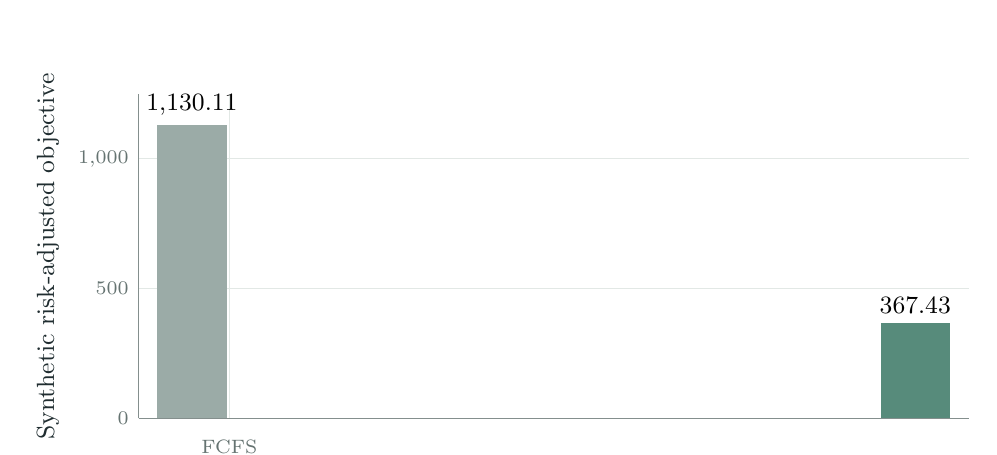
\begin{tikzpicture}
\begin{axis}[cleanbar,width=\linewidth,height=5.7cm,symbolic x coords={FCFS,GlobalMILP},xtick=data,ymin=0,ymax=1250,ylabel={Synthetic risk-adjusted objective},bar width=25pt,nodes near coords,nodes near coords style={font=\small}]
\addplot[fill=silver,draw=none] coordinates {(FCFS,1130.1063)};
\addplot[fill=sage,draw=none] coordinates {(GlobalMILP,367.4283)};
\end{axis}
\end{tikzpicture}\par\vspace{2mm}
\begin{insight}
A single constructed capacity-conflict fixture gave a \textbf{67.5\%} lower synthetic risk-adjusted objective for global MILP versus FCFS. This is a \emph{stress fixture}, not an average across an operating airline network. In the default live v10 network evaluations at ticks 0, 4, 8 and 12, the MILP and FCFS benchmarks reported \textbf{0\%} incremental saving.
\end{insight}
\subsect{Finite-route MILP runtime (36 recorded solves)}
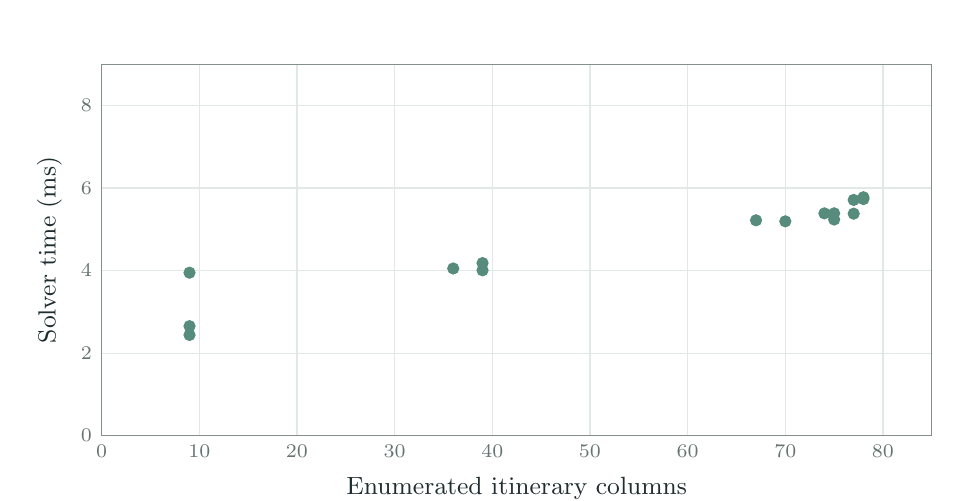
\begin{tikzpicture}
\begin{axis}[replot,width=\linewidth,height=6.3cm,xmin=0,xmax=85,ymin=0,ymax=9,xlabel={Enumerated itinerary columns},ylabel={Solver time (ms)}]
% Representative raw measurements from the 36-run runtime CSV.
\addplot[only marks,mark=*,mark size=2pt,color=sage] coordinates {(9,3.949)(39,4.182)(70,5.193)(78,5.777)(75,5.237)(77,5.712)(9,2.654)(36,4.051)(67,5.218)(78,5.733)(75,5.387)(77,5.379)(9,2.441)(39,4.007)(74,5.386)};
\end{axis}
\end{tikzpicture}\par
\methodnote{Displayed: 15 representative observations from the measured set of 36; previously reported median 5.31 ms, p95 6.20 ms, solver statuses optimal with MIP gap 0. This is not a large-network scalability guarantee.}
\subsect{Recovery-speed counterexample (temporary disruption)}
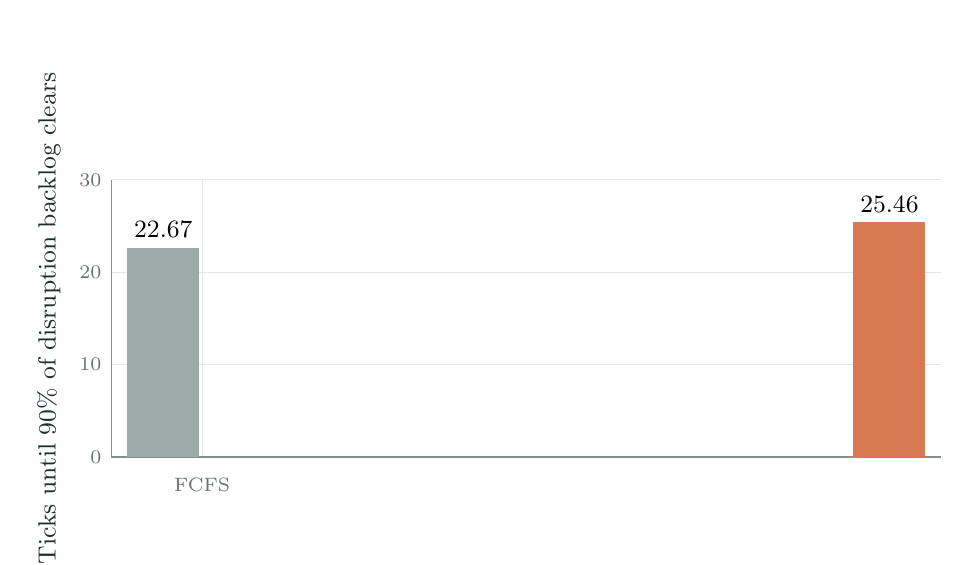
\begin{tikzpicture}
\begin{axis}[cleanbar,width=\linewidth,height=5.1cm,symbolic x coords={FCFS,ModelA},xtick=data,ymin=0,ymax=30,ylabel={Ticks until 90\% of disruption backlog clears},bar width=26pt,nodes near coords,nodes near coords style={font=\small}]
\addplot[fill=silver,draw=none] coordinates {(FCFS,22.67)};
\addplot[fill=coral,draw=none] coordinates {(ModelA,25.46)};
\end{axis}
\end{tikzpicture}\par
\risk{Model A takes about 12.3\% longer to clear this backlog threshold.} Lower average synthetic cost does not imply faster backlog recovery.\par
\newpage

% -------------------------- SPEED / TWIN -------------------------
\sect{10 / Digital Twin and runtime QA}{REAL-TIME MEANING}
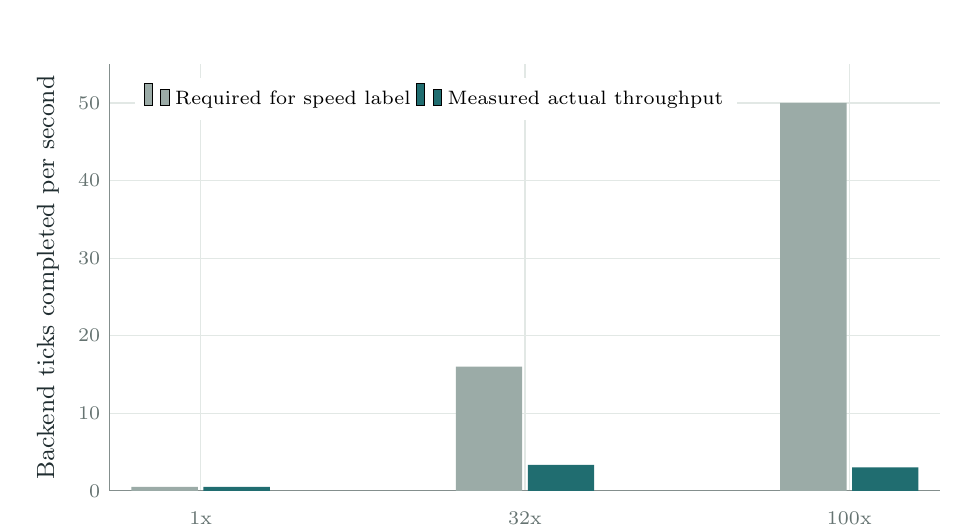
\begin{tikzpicture}
\begin{axis}[cleanbar,width=\linewidth,height=7cm,symbolic x coords={1x,32x,100x},xtick=data,ymin=0,ymax=55,ylabel={Backend ticks completed per second},bar width=24pt,legend pos=north west]
\addplot[fill=silver,draw=none] coordinates {(1x,.5)(32x,16)(100x,50)};\addlegendentry{Required for speed label}
\addplot[fill=teal,draw=none] coordinates {(1x,.499)(32x,3.356)(100x,3.012)};\addlegendentry{Measured actual throughput}
\end{axis}
\end{tikzpicture}\par\vspace{2mm}
\begin{tabularx}{\linewidth}{@{}lrrr@{}}
\toprule
User setting & Requested ticks/s & Measured ticks/s & Achieved fraction\\\midrule
1$\times$ & 0.500 & 0.499 & 99.8\%\\
32$\times$ & 16.000 & 3.356 & 21.0\%\\
100$\times$ & 50.000 & 3.012 & 6.0\%\\
\bottomrule
\end{tabularx}
\methodnote{Short wall-clock windows from v10 QA; sensitive to host CPU, solver workload and measurement overhead. More rapid animation is not proof of 100$\times$ numerical simulation throughput.}
\subsect{Cross-Twin integration checks}
\begin{tabularx}{\linewidth}{@{}p{40mm}X@{}}
\toprule
Customer $\rightarrow$ Ground & A new synthetic HKG--NRT 135 kg order appears with shared shipment identity in the staging/catalogue view.\\
Ground $\rightarrow$ Tower & Tick advance and disruption event update the shared versioned state; a dimension conflict triggers an uncertainty gate.\\
Tower $\rightarrow$ Customer & Affected order shows a disruption-observed journey event; proposed route does not become externally booked merely because it is internally approved.\\
UI + API & Three views rendered in Chromium QA; eight important HTTP GET/POST routes returned 200 in v10 audit.\\
Security & Unauthenticated local sandbox control mutation was permitted; unacceptable for public multi-tenant deployment.\\
\bottomrule
\end{tabularx}
\begin{caution}
\textbf{Shared state is not a certified physical digital twin.} Simulated vehicle/aircraft poses, routes and weather displays are procedural projections. Real-world causality would need authenticated ground-task, ULD, custody, ETA and equipment telemetry with timestamps and replay.
\end{caution}
\newpage

% -------------------------- SCENARIO WEIGHTS ---------------------
\sect{11 / Probability-weighted expected cost}{ILLUSTRATIVE MIX, NOT OBSERVED FREQUENCY}
The following scenario weights are \textbf{hypothetical}, chosen only to demonstrate how to aggregate synthetic costs: Normal 40\%, Peak 20\%, Crew shortage 15\%, Cold outage 10\%, High capacity 10\%, Disruption 5\%.
\[
\mathbb E[C_{\pi}]=\sum_{s=1}^{6}p_s\,\overline C_{\pi,s},\qquad
\text{Saving}_{\pi}=100\Bigl(1-\frac{\mathbb E[C_\pi]}{\mathbb E[C_{\rm FCFS}]}\Bigr)\%.
\]
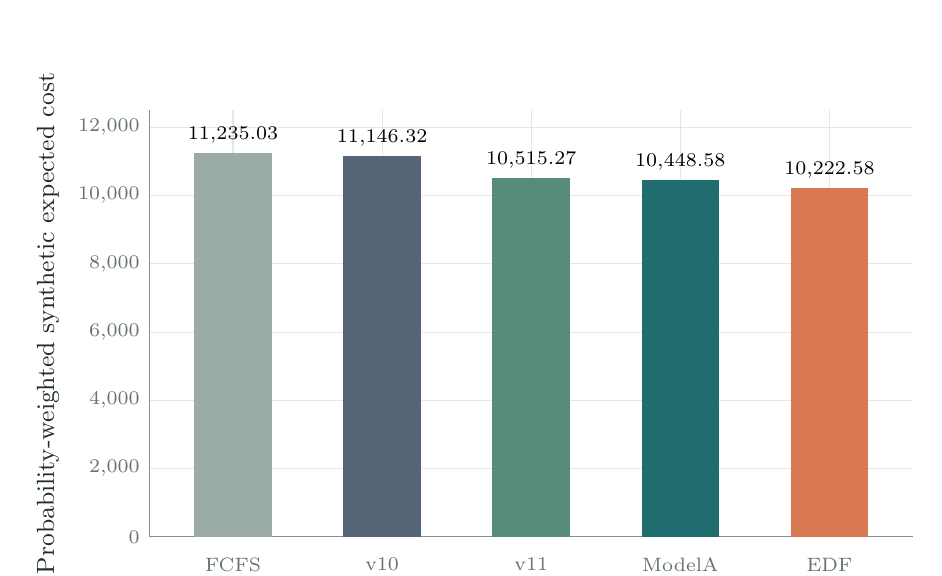
\begin{tikzpicture}
\begin{axis}[cleanbar,width=.93\linewidth,height=7cm,symbolic x coords={FCFS,v10,v11,ModelA,EDF},xtick={FCFS,v10,v11,ModelA,EDF},ymin=0,ymax=12500,ylabel={Probability-weighted synthetic expected cost},bar width=28pt,nodes near coords,nodes near coords style={font=\scriptsize,rotate=0,anchor=south}]
\addplot[fill=silver,draw=none,bar shift=0pt] coordinates {(FCFS,11235.030)};
\addplot[fill=slate,draw=none,bar shift=0pt] coordinates {(v10,11146.321)};
\addplot[fill=sage,draw=none,bar shift=0pt] coordinates {(v11,10515.272)};
\addplot[fill=teal,draw=none,bar shift=0pt] coordinates {(ModelA,10448.577)};
\addplot[fill=coral,draw=none,bar shift=0pt] coordinates {(EDF,10222.576)};
\end{axis}
\end{tikzpicture}\par\vspace{2mm}
\begin{tabularx}{\linewidth}{@{}Xrr@{}}
\toprule
Policy & Hypothetical expected synthetic cost & Saving vs FCFS\\\midrule
FCFS & 11,235.03 & 0\%\\
RELAY v10 & 11,146.32 & 0.79\%\\
RELAY v11 & 10,515.27 & 6.41\%\\
RELAY + Model A & 10,448.58 & \good{7.00\%}\\
RELAY + EDF & 10,222.58 & \good{9.01\%}\\
\bottomrule
\end{tabularx}
\begin{caution}
The percentages in this section are \textbf{not unconditional observed savings}. Changing the six scenario probabilities can change the weighted ranking and aggregate improvement. Never present these assumed weights as the historical frequency of Cathay Cargo operations.
\end{caution}
\newpage

% -------------------------- ROI ----------------------------------
\sect{12 / ROI and break-even sensitivity}{HYPOTHETICAL ECONOMICS ONLY}
\[
\Delta C = C_{\rm FCFS}-C_{\rm Model\ A}=1946.835-1723.600=\boxed{223.235\text{ synthetic units/episode}}.
\]
\[
\text{Net monthly benefit}=N\,k\,\Delta C-F,\qquad
\boxed{\mathrm{ROI}(\%)=100\frac{Nk\Delta C-F}{F}},\qquad
\boxed{k_{\rm BE}=\frac{F}{N\Delta C}}.
\]
\begin{tabularx}{\linewidth}{@{}p{21mm}X@{}}
$N$ & Monthly comparable episodes; \emph{user-assumed}, not inferred from Cathay's real demand.\\
$k$ & Hypothetical HKD value of one synthetic penalty unit. \emph{Not calibrated.}\\
$F$ & Monthly incremental total deployment/operating cost, here set to HKD 20,000 \emph{for illustration only}.\\
\end{tabularx}
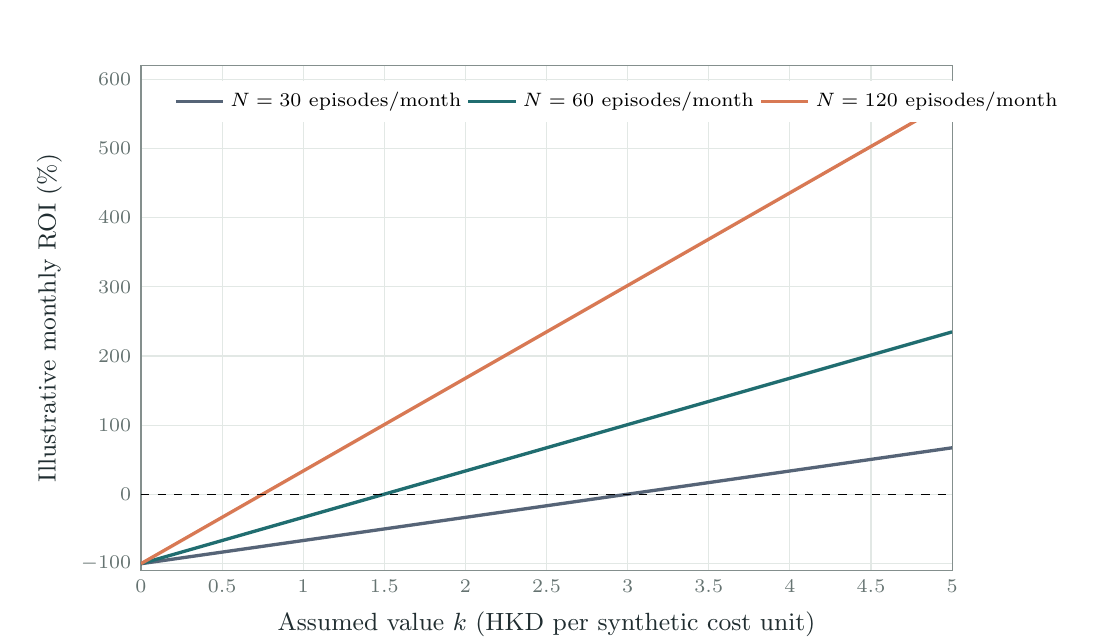
\begin{tikzpicture}
\begin{axis}[replot,width=.98\linewidth,height=8cm,xmin=0,xmax=5,ymin=-110,ymax=620,xlabel={Assumed value $k$ (HKD per synthetic cost unit)},ylabel={Illustrative monthly ROI (\%)},legend pos=north west]
\addplot[very thick,slate,domain=0:5,samples=70] {100*((30*223.235*x-20000)/20000)};\addlegendentry{$N=30$ episodes/month}
\addplot[very thick,teal,domain=0:5,samples=70] {100*((60*223.235*x-20000)/20000)};\addlegendentry{$N=60$ episodes/month}
\addplot[very thick,coral,domain=0:5,samples=70] {100*((120*223.235*x-20000)/20000)};\addlegendentry{$N=120$ episodes/month}
\addplot[black,dashed,domain=0:5] {0};
\end{axis}
\end{tikzpicture}\par\vspace{2mm}
\begin{tabularx}{\linewidth}{@{}lrrrrr@{}}
\toprule
Monthly episodes & $k=0.5$ & $k=1$ & $k=2$ & $k=5$ & Break-even $k$\\\midrule
30 & --83.3\% & --66.5\% & --33.0\% & +67.4\% & HKD 2.99\\
60 & --66.5\% & --33.0\% & +33.9\% & +234.9\% & HKD 1.49\\
120 & --33.0\% & +33.9\% & +167.9\% & +569.7\% & HKD 0.75\\
\bottomrule
\end{tabularx}
\begin{caution}
\textbf{Actual currency ROI cannot yet be identified.} The numbers depend critically on $k$, $F$, volume, adoption, operational constraints and whether the synthetic gain persists on real data. No causal field study or calibrated monetary cost ledger exists. This chart is a \emph{decision threshold model}, not a savings forecast.
\end{caution}
\newpage

% -------------------------- PRODUCTION GAPS ----------------------
\sect{13 / QA findings and production gaps}{ACTIONABLE HANDOVER}
\begin{tabularx}{\linewidth}{@{}p{33mm}X>{\centering\arraybackslash}p{19mm}@{}}
\toprule
Gap & Why it matters & Priority\\\midrule
Real cargo and OAG data & Synthetic schema quality does not establish actual delay, cost or connection probability. OAG schedules cannot certify remaining cargo capacity. & High\\
Full 3D safety & 2D floor fit and box preflight miss contour, restraint, balance and handling trajectory. & Critical\\
Sequential Bayes & Verification decisions lack fully coupled time-dependent beliefs and complete counterfactual route re-optimisation. & High\\
Global re-optimisation & HOLD/VERIFY can release capacity that the system should reassess globally. & High\\
Network candidate space & Finite itinerary enumeration need not contain the real-world best itinerary. & High\\
Cluster exchange method & Mathematical mutation visualisation is not a production Graver-basis algorithm. & Research\\
Benchmark horizon & End-of-window unfinished jobs must enter SLA and cost; full-cohort v11 improves this. & Addressed\\
Worst-case operations & Severe crew shortage has 0\% gain under fallback; recovery backlog can clear more slowly. & High\\
Engineering security & Sandbox endpoints lack real authentication and role-level isolation. & Critical\\
Throughput & 100$\times$ labelled playback did not deliver 100$\times$ backend computation in v10 QA. & Medium\\
\bottomrule
\end{tabularx}
\subsect{A narrow, credible shadow-mode pilot}
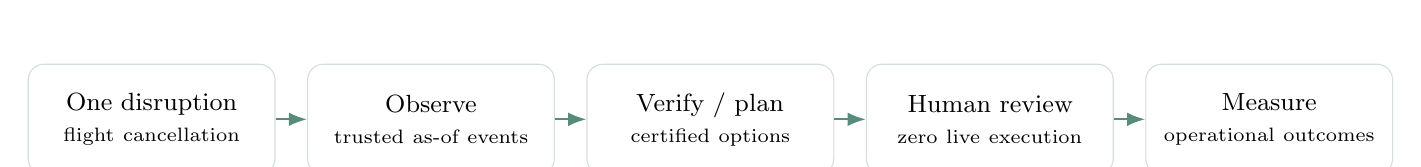
\begin{tikzpicture}[node distance=2mm,>=Latex,every node/.style={font=\small}]
\tikzset{p/.style={draw=line,fill=white,rounded corners=2mm,align=center,text width=29mm,minimum height=14mm}}
\node[p] (one) {One disruption\\\scriptsize flight cancellation};
\node[p,right=4mm of one] (two) {Observe\\\scriptsize trusted as-of events};
\node[p,right=4mm of two] (three) {Verify / plan\\\scriptsize certified options};
\node[p,right=4mm of three] (four) {Human review\\\scriptsize zero live execution};
\node[p,right=4mm of four] (five) {Measure\\\scriptsize operational outcomes};
\foreach \a/\b in {one/two,two/three,three/four,four/five}{\draw[->,thick,sage] (\a)--(\b);}
\end{tikzpicture}\par\vspace{2mm}
\begin{insight}
\textbf{Recommended final positioning.} RELAY is a \emph{working, auditable, synthetic decision-support prototype} with measurable scenario-dependent scheduling potential. It is sufficiently mature to demonstrate the hypothesis of purchasing future optionality, but not yet to make a numerical claim about real cargo-line savings. Stop major UI feature expansion; prioritise pilot-grade data, objective weights, recovery-clearance constraints and security.
\end{insight}
\newpage

% -------------------------- METHODOLOGY --------------------------
\sect{14 / Definitions, method and evidence}{REPRODUCIBILITY NOTES}
\subsect{Metric definitions}
\begin{align*}
\text{Cost saving }(\%) &=100\,\frac{\overline C_{\mathrm{FCFS}}-\overline C_{\pi}}{\overline C_{\mathrm{FCFS}}},\\[2pt]
\text{On-time rate }(\%)&=100\,\frac{\#\text{jobs meeting due-time criterion}}{\#\text{all admitted jobs}},\\[2pt]
\text{On-time gain }(\mathrm{pp})&=\mathrm{OTR}_{\pi}-\mathrm{OTR}_{\mathrm{FCFS}},\\[2pt]
\text{Lead time reduction }(\%)&=100\,\frac{\overline T_{\mathrm{FCFS}}-\overline T_{\pi}}{\overline T_{\mathrm{FCFS}}},\\[2pt]
\mathrm{CVaR}_{\alpha}(C)&=\min_{\eta\in\mathbb R}\left\{\eta+\frac{1}{1-\alpha}\,\mathbb E[(C-\eta)_+]\right\},\\[2pt]
\text{Policy regression rate }(\%)&=100\,\frac{\#\{e:C_\pi(e)>C_{\mathrm{FCFS}}(e)\}}{\#\text{paired episodes}}.
\end{align*}
\subsect{Test configurations and QA provenance}
\begin{tabularx}{\linewidth}{@{}p{38mm}X@{}}
\toprule
Holdout & Seed 9099; six regimes; 500 common episodes per regime; five policies; 15,000 episode--policy records.\\
Development split & Seed 707, 55 episodes/regime for experimental hybrid policy exploration; holdout subsequently evaluated separately.\\
Earlier v11 release QA & Seed 2026, 500 paired episodes/regime, two recorded RELAY policies, full-cohort clearance horizon.\\
Legacy v10 QA & 124/124 tested in separate regression groups; an earlier staging benchmark had shorter, potentially censored horizon.\\
Safety QA & Zero safety violations \emph{in checked synthetic policy assignments}; the result is not real ULD certification.\\
Microbenchmark & 50 waiting jobs / 500 timing repetitions: median selection 0.0072 ms (FCFS), 0.0363 ms (v11), 0.0346 ms (Model A). These exclude the full engine and browser.\\
Data fields & Source code reports include event timestamp, receipt timestamp, snapshot version, shipment identifier and action provenance; no cryptographically tamper-evident production log attestation.\\
\bottomrule
\end{tabularx}
\subsect{Source artefacts (local experiment outputs)}
\begin{itemize}
\item \texttt{RELAY\_HYBRID\_HOLDOUT\_SUMMARY.csv}: all 30 strategy-by-regime summary rows.
\item \texttt{RELAY\_HYBRID\_HOLDOUT\_EPISODES.csv}: all 15,000 hybrid experiment outcomes.
\item \texttt{RELAY\_HYBRID\_HOLDOUT\_RESULTS.json}: seed, policy descriptions, and statistical convergence traces.
\item \texttt{V11\_PRESENTATION\_KPIS.csv}: release v11 seed-2026 cohort metrics, kept separate from hybrid holdout.
\item \texttt{V11\_FINITE\_MILP\_RUNTIME.csv}: 36 recorded finite MILP timings.
\item \texttt{RELAY\_QA\_v10\_measured\_data.csv}: five-regime legacy QA outcomes.
\end{itemize}
\begin{caution}
\textbf{External-validity boundary.} All plotted results are from local synthetic data or explicitly hypothetical economics. The report makes no claim to know Cathay's real shipment statistics, live OAG credentials, remaining booking inventory, monetary cost function, safety certificates, or a causal field-effect estimate.
\end{caution}
\vfill
\begin{center}
{\sffamily\Large\bfseries THE CASE IS PROMISING. THE FIELD ROI IS STILL UNPROVEN.}\\[4mm]
{\small\color{muted} RELAY / Research-to-product QA / End of report}
\end{center}
\end{document}
